%!TEX root = ProgCPP_ZF.tex

\part{Überladen von Operatoren (Operator overloading)}
\label{sec:operator overloading}
Überladen ist hier nicht im Sinne von "zu viel laden" zu verstehen, sondern im Sinne von "drüber laden", "zudecken", "neu definieren".\\
Mit Operator overloading kann ein bestehender Operator neu definiert (überladen) werden.

\section{Operator overloading in C++}
\begin{itemize}
	\item Spezialität von C++ (wurde auch in C\# aufgenommen, nicht aber in Java)
	\item Operatoren (z.B. +, ==, etc.) können wie Funktionen überladen werden, z.B.
	\begin{itemize}
		\item Der Operator + kann bei einer String-Klasse sehr praktisch sein, um zwei Strings aneinanderzufügen.
		\item Der Operator + kann definiert werden, um zwei Matrizen oder zwei komplexe Zahlen zu addieren.
		\item Der Operator << kann für eine neue Klasse definiert werden, um auch Objekte dieser Klasse auf cout schreiben zu können. Damit können neue Klassen nahtlos in das bestehende C++-System integriert werden.
	\end{itemize}
	\item Operator overloading ist zwar nicht sehr objektorientiert aber enorm praktisch.
\end{itemize}
\vspace{\baselineskip}
\textbf{Überladbare (overloadable) Operatorfunktionen in C++}\\
\vspace{\baselineskip}
\begin{tabular}{|l|c|c|c|c|}
	\hline 
	new & delete & new[] & delete[] &  \\ 
	+ & - & * & / & \% \\ 
	\hline 
	$\textasciicircum$ & \& & | & ~ & ! \\ 
	\hline 
	= & < & > & += & -= \\ 
	\hline 
	*= & /= & \%= & $\textasciicircum=$ & \&= \\ 
	\hline 
	|= & << & >> & >>= & <<= \\ 
	\hline 
	== & != & <= & >= & \&\& \\ 
	\hline 
	|| & ++ & -- & , & ->* \\ 
	\hline 
	-> & () & [] &  &  \\ 
	\hline 
\end{tabular}

\subsection{Operatorfunktion}
Die erwähnten Operatoren sind in C++ mit einer Operatorfunktion implementiert, d.h. im Hintergrund wird eigentlich eine Funkion aufgerufen.\\
Die Operatoren können sowohl in der üblichen Operatornotation als auch in der Funktionsnotation verwendet werden.
\vspace{\baselineskip}
\textbf{Beispiel: ein String zu einem bestehenden String addieren}\\
Operatornotation (üblich): str3+= str2;\\
\vspace{\baselineskip}
Funktionsnotation (alternativ, unüblich): str3.operator +=(str2);

\subsection{Randbedingungen zu Operator overloading}
\begin{itemize}
	\item Die Anzahl der Operanden (Argumente) muss gleich sein wie beim ursprünglichen Operator
	\item Die Priorität des überladenen Operators kann nicht ändern
	\item Neue Operatoren können nicht eingeführt werden
	\item Default-Argumente sind bei Operatoren nicht möglich
	\item nicht gefordert aber sinnvoll: die neue Operation sollte intuitiv dem bestehenden Operator zugeordnet werden können
\end{itemize}
\vspace{\baselineskip}
\subsection{Umsetzungsvarianten für Operator overloading}
\begin{itemize}
	\item Operator overloading als Elementfunktion
	\begin{itemize}
		\item Zwingend für folgende Operatoren
		\begin{itemize}
			\item{\makebox[4cm]{Zuweisung\hfill}} =
			\item {\makebox[4cm]{Index\hfill}} []
			\item {\makebox[4cm]{Funktionsaufruf\hfill}} ()
			\item {\makebox[4cm]{Zeigeroperator\hfill}} ->
		\end{itemize}
	\end{itemize}
	\item Operator overloading als "normale"  Funktion
	\begin{itemize}
		\item Typischerweise für alle anderen
	\end{itemize}
\end{itemize}
\begin{multicols}{2}
	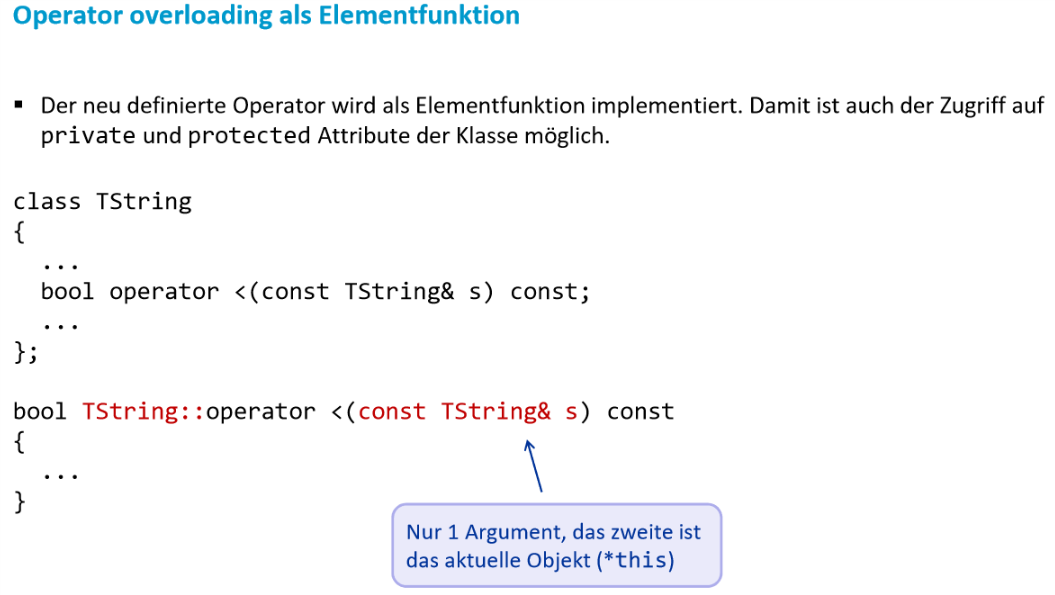
\includegraphics[width=\linewidth]{images/operatorOverloading.png}
	\columnbreak
	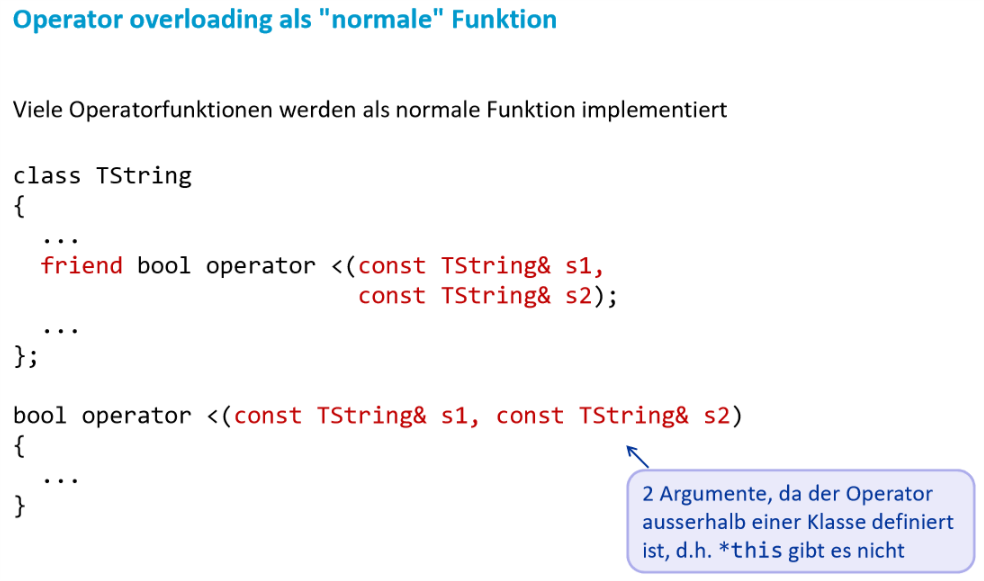
\includegraphics[width=\linewidth]{images/operatorOverloadingNormaleFunktion.png}
\end{multicols}
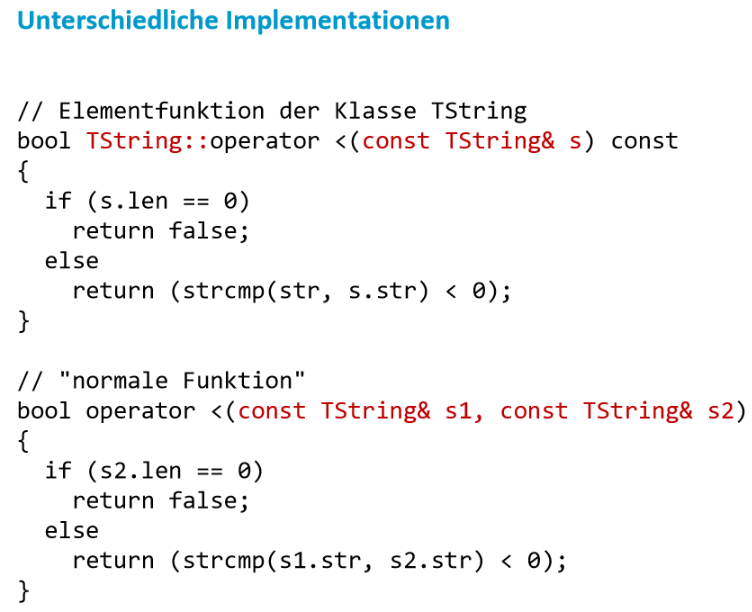
\includegraphics[width=\linewidth]{images/operatorOverloadingBeide.png}

\subsubsection{Beispiel}
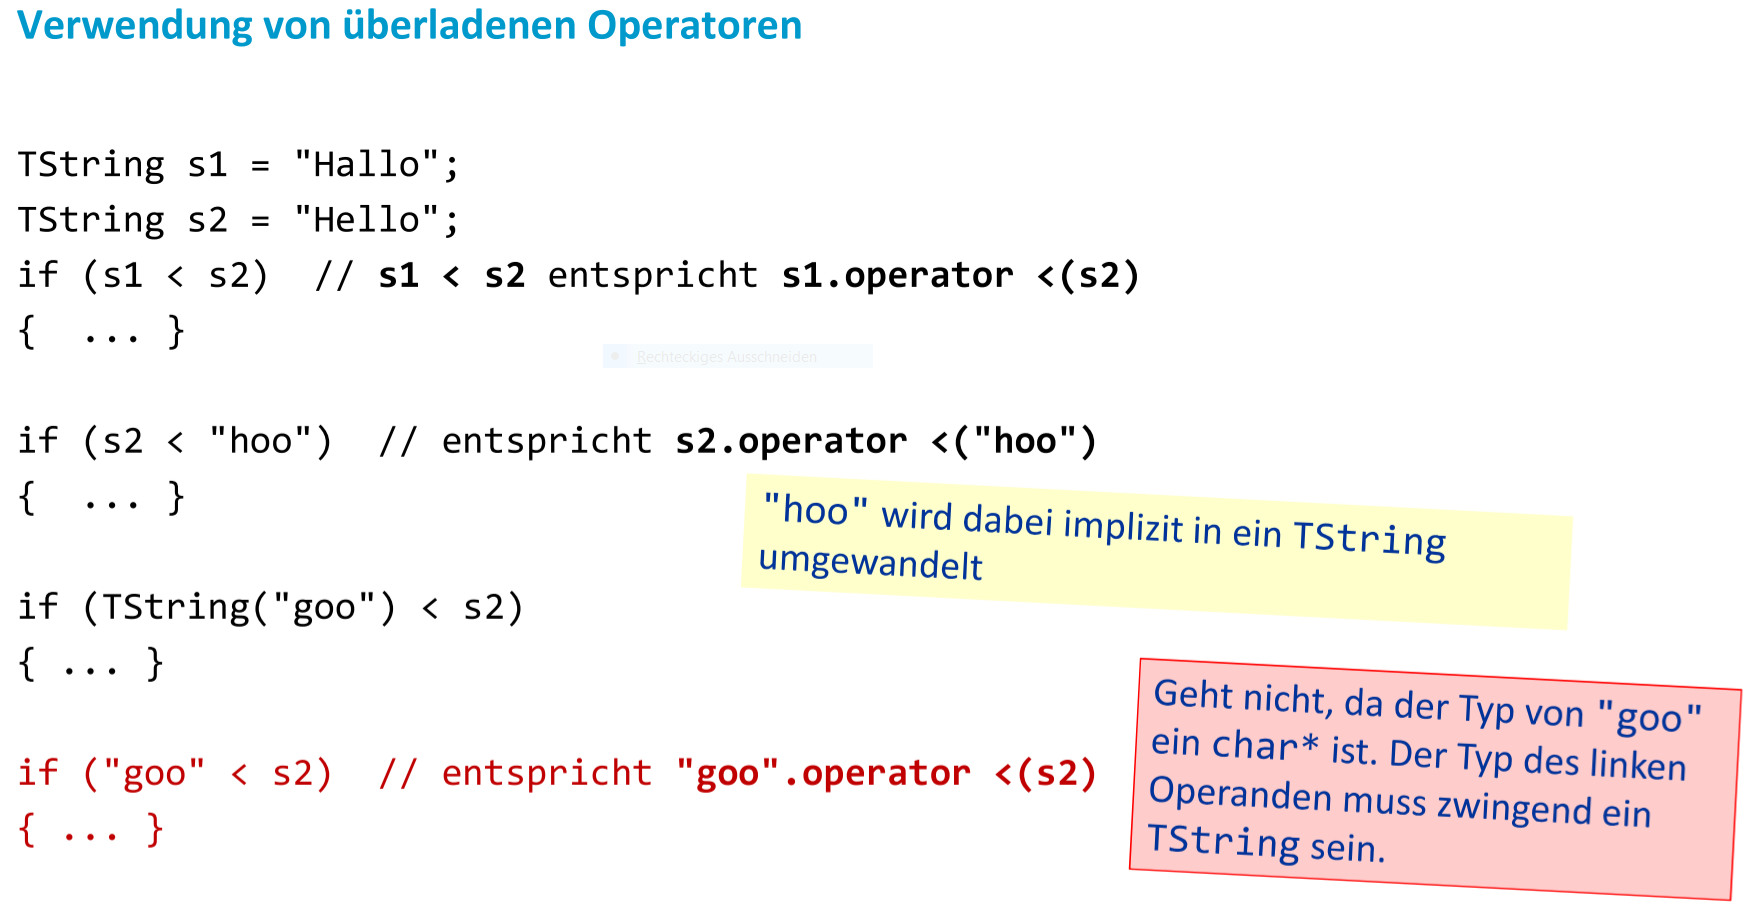
\includegraphics[width=\linewidth]{images/verwendung.png}
Problemlösung:
\begin{itemize}
	\item Ich möchte den Operator unbedingt auch so verwenden können:
	\noindent
	\item[\-]\vspace{-\baselineskip}\begin{minipage}{\linewidth}
	\begin{lstlisting}
	if("goo" < s2)
	{...}
	\end{lstlisting}
	\end{minipage}
	\item Da der linke Operator zwingend ein Objekt der Klasse sein muss, geht das so nicht.
	\item Lösung:
	\begin{itemize}
		\item Die Operatorfunktion wird nicht als Elementfunktion der Klasse definiert sondern als "normale" Funktion ausserhalb der Klasse.
		\item Dadurch besteht jedoch kein Zugriff mehr auf die private und protected Elemente der Klasse
		\item Die Operatorfunktion muss deshalb als friend deklariert werden (dies ist auch praktisch die einzige $"$erlaubte$"$ Verwendung von friend)
	\end{itemize}
\end{itemize}

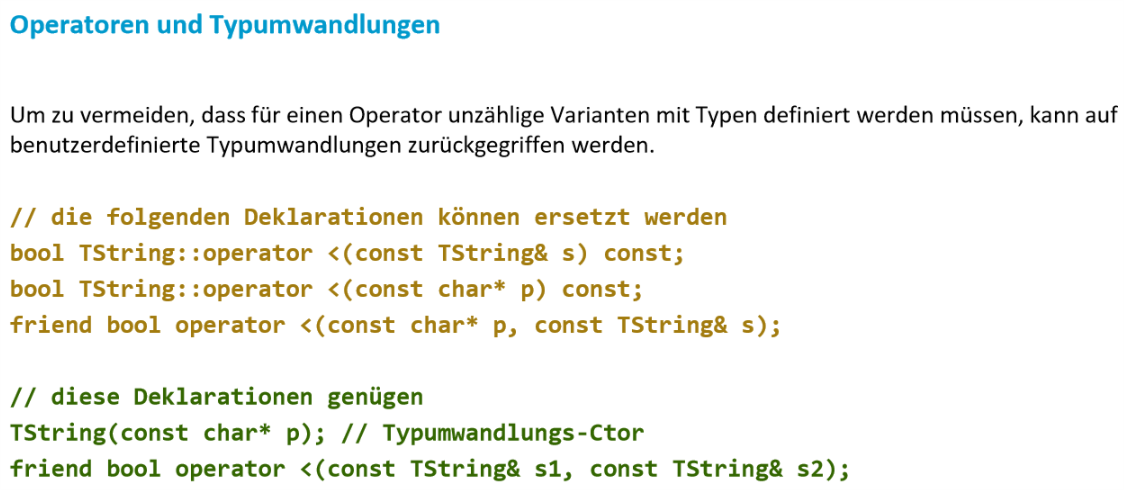
\includegraphics[width=\linewidth]{images/operatorenTypumwandlungen.png}

\subsubsection{Zuweisungsoperator =}
\label{sec:zuweisungsoperator}
\noindent
\begin{minipage}{\linewidth}
	\begin{lstlisting}
	TString& TString::operator=(const TString& s)
	{
		if (this == &s)
			return *this;	// "a1 = a1"
		
		delete[] str;	// alte Inhalte loeschen
		str = 0;
		
		len = s.len;	// neu allokieren und kopieren
		if (s.str != 0)
		{
			str = new char[len+1];
			memcpy(str, s.str, len+1);
		}
		return *this;
	}
	\end{lstlisting}
\end{minipage}

\subsubsection{Indexoperator []}
\begin{itemize}
	\item Wir möchten auf einen einzelnen Buchstaben eines TString-Objekts mittels Indexoperator 	zugreifen können:
	\noindent
	\item[\-]\vspace{-\baselineskip}\begin{minipage}{\linewidth}
		\begin{lstlisting}
		TString s = "Hallo";
		s[2] = 'h';
		char ch = s[3];
		\end{lstlisting}
	\end{minipage}
	\item Dies kann durch die explizite Implementation des Indexoperators in der Klasse TString erreicht werden
	\item Die Operatorfunktion soll eine Referenz auf das gewünschte Zeichen zurückgeben, d.h. ein char\&
	\subitem \textbf{char\& operator[](int pos);}
	\item Wieso braucht es zwei Varianten?
	\item[\-] char\& operator[](int pos);
	\item[\-] const char\& operator[](int pos) const;
	\noindent
	\item[\-]\vspace{-\baselineskip}\begin{minipage}{\linewidth}
		\begin{lstlisting}
		char& operator[](int pos);
		TString s = "Hallo";
		s[2] = 'h';
		char ch = s[3];
		
		void foo(const TString& s)	
		{
			char ch = s[4];
		}
		\end{lstlisting}
		\color{red}foo-Funktion geht mit erster Variante nicht!\color{black}\\Mit einem const-Objekt können nur const-Methoden aufgerufen werden. Deshalb braucht es auch die zweite Variante.
	\end{minipage}
\end{itemize}

\subsubsection{Beispiel Klasse TString}
\begin{itemize}
	\item{\makebox[4cm]{Indexoperator\hfill}} []
	\item{\makebox[4cm]{Operator\hfill}} ()
	\item{\makebox[4cm]{Zuweisungsoperator\hfill}} =
	\item[\-] (Achtung: shallow vs. deep copy)
	\item Typumwandlungsoperator nach char*
	\item{\makebox[4cm]{Vergleichsoperatoren\hfill}} ==\quad!=\quad<\quad>
	\item{\makebox[4cm]{Verkettungsoperatoren\hfill}} +\quad+=
\end{itemize}

\subsubsection{Eigenen Zuweisungsoperator definieren}
Wie beim Copy Konstruktor gilt auch für den Zuweisungsoperator:\\
Wenn die Klasse Elemente auf dem Heap unterhält, dann muss der Zuweisungsoperator selbst definiert werden, damit eine Deep Copy erstellt wird.

\subsubsection{Zur Erinnerung: Kanonische Form einer Klasse}
\begin{itemize}
	\item Wenn eine Klasse in der kanonischen Form vorliegt, dann kann sie verwendet werden wie ein "normaler Typ"
	\item Um das zu erreichen, müssen bei Klassen, welche Speicher auf dem Heap unterhalten, die folgenden Elemente definiert werden:
	\begin{itemize}
		\item Copy Konstruktor
		\item Destruktor
		\item Zuweisungsoperator
	\end{itemize}
\end{itemize}

\subsection{Streamkonzept}
\label{sec:streamkonzeptOverloading}
(\emph{siehe \ref{sec:streamkonzept}})

\subsubsection{Ausgabe: Klasse ostream}
\begin{itemize}
	\item \emph{(siehe \ref{sec:ostream})}
	\item Nutzung mit cout (vordefiniertes Objekt der Klasse ostream):\\
	int i = 45;\\
	cout << "Hallo " << i << endl;\\
	TString s;\\
	\color{red}cout << s;\qquad//funktioniert nicht, wenn Operator nicht überladen \color{black}
\end{itemize}

\subsubsection{Operator << überschreiben}
\noindent
\begin{minipage}{\linewidth}
\begin{lstlisting}
class TString
{
	public:
		...
		friend ostream& operator <<(ostream& os, const TString& s);
		...
};

ostream& operator <<(ostream& os, const TString& s)
{
	if (s.str != 0)
		return os << s.str;		// s.str ist char*
	else
		return os
}
\end{lstlisting}
\end{minipage}

\subsubsection{Eingabe: Klasse istream}
\begin{itemize}
	\item \emph{(siehe \ref{sec:istream})}
	\item Nutzung mit cin (vordefiniertes Objekt der Klasse istream):\\
	double d;\\
	string str;\\
	cin >> d >> str;\\
	TString s;\\
	\color{red}cint >> s;\qquad// funktioniert nicht, wenn Operator nicht überladen \color{black}
\end{itemize}

\subsubsection{Operator >> überschreiben}
\noindent
\begin{minipage}{\linewidth}
\begin{lstlisting}
class TString
{
	public:
		...
		friend istream& operator >>(istream& is, const TString& s);
		...
};

char buffer[stringSize];	// statisch allokierter Eingabebuffer
istream& operator >>(istream &is, TString &s)
{
	is >> buffer;		// in statische Buffer lesen
	s = buffer;		// dann nach s kopieren
	return is;
}
\end{lstlisting}
\end{minipage}